%
%  == Collective paper on MORSE for HRI ==
%
%
% Editing of the article moves to GIT (Sharelatex does not expose the change history unless you
% pay for it, so it's difficult to track changes and merge them with GIT).
%
% The repo is here:  https://github.com/morse-simulator/publication-iros2014-hri
%
%
% The idea is: each of you present (in one section) its project, 
% putting an emphasis on:
%   1- why simulation is useful/needed for your use-case
%   2- is it satisfactory or not
%   3- what is good and could be useful to other researcher
%   4- what is missing both at the technical level (things that could be added 
%      to MORSE) and at a more fundamental level (things where simulation do 
%      not fit)
%
% It would be great to have one nice screenshot per project.
%
% Then, Severin and Florian write a synthesis in the conclusion.
%
% Severin will also write a short introduction + presentation of MORSE for HRI
%


\documentclass[conference]{IEEEtran}

% UTF8 support
\usepackage[utf8x]{inputenc}
\usepackage[T1]{fontenc}
\usepackage{url}
\usepackage{graphicx}
\usepackage{float}
\graphicspath{{figs/}}
\newcommand{\eg}{{\textit{e.g.~}}}
\newcommand{\etal}{{\textit{et al.~}}}
\newcommand{\ie}{{\textit{i.e.~}}}

\begin{document}

\title{Simulation and HRI: Recent Perspectives}
% I suggest for now to keep the authors in alphabetic order.
% Please add yourself!

\author{\IEEEauthorblockN{
Michael Karg\IEEEauthorrefmark{4},
Harmish Khambhaita\IEEEauthorrefmark{1},
Lars Kunze\IEEEauthorrefmark{5},
Séverin Lemaignan\IEEEauthorrefmark{2},
Florian Lier\IEEEauthorrefmark{3},
Ingo Lütkebohle\IEEEauthorrefmark{4} and
Grégoire Milliez\IEEEauthorrefmark{1}
\IEEEauthorblockA{\IEEEauthorrefmark{1}Laboratoire d'Analyse et d'Architecture des Système,
Université de Toulouse,
Toulouse, France}
\IEEEauthorblockA{\IEEEauthorrefmark{2}Computer-Human Interaction for Learning and Instruction,
École Polytechnique Fédérale de Lausanne,
Lausanne, Switzerland}
\IEEEauthorblockA{\IEEEauthorrefmark{3}Cognitve Interaction Technology --- Center of Excellence,
Bielefeld University, Bielefeld, Germany}
\IEEEauthorblockA{\IEEEauthorrefmark{4}Institute for Advanced Study, Technische Universit\"{a}t M\"{u}nchen, D-85748 Garching, Germany}
\IEEEauthorblockA{\IEEEauthorrefmark{5}Intelligent Robotics Lab, School of Computer Science, University of Birmingham, United Kingdom}
}}


\maketitle

\begin{abstract}

Simulation in robotics is often a love-hate relationship: while simulators do
save us a lot of time and effort compared to regular deployment of complex
software architectures on complex hardware, simulators are also known to evade
many (if not most) of the very real issues that robots need to manage when they
enter the real world.  Because humans are the paragon of dynamic, unpredictable,
complex, real world entities, simulation of human-robot interactions may look
condemn to fail, or, in the best case, to be largely useless.  This collective
article reports on five unrelated and actually very different applications of
the MORSE simulator related to human-robot interaction: It appears that
simulation is already useful (and even essential in some case) to successfully
carry out research in the field of HRI, be it for not-so-expected reasons.

\end{abstract}

\IEEEpeerreviewmaketitle

\section{Introduction}

% We should def. list a few requirements here, based on our experience

This article attempts to provide feedback from field experiences with simulation
for human-robot interaction. The originality of this contribution lies into its
collective nature. We report here contributions and experiences from five
unrelated projects, conducted by different people in different universities and
research institutes. These projects share however one common tool: they all use
the MORSE simulator as simulation platform.

The sections~\ref{scenario1} to~\ref{scenario5} present each of these projects,
and try to shed some light on the positive outcomes of deploying simulation
environments for HRI, as well as the pitfalls and more fundamental issues that
simulation of human-robot interaction still faces.

\subsection*{HRI and simulation}

% Also mention the focus of simulation so far: Physics, Kinematics, Actuator simulation a human component
% has been neglected to far See also Comment below for related work [flier] -->

% Mention Gazebo "animated characters": http://gazebosim.org/wiki/Tutorials/intermediate/animated_characters 
Other experiments using simulation have been carried to gather data for HRI
\cite{Chernova2011}. However, these do not involve the actual robot software,
and it is another human who takes the role of the robot.

\subsection*{HRI and the MORSE simulator}

The five projects that are presented in this article all rely on the Modular
OpenRobots Simulation Engine (MORSE)~\cite{Echeverria2011, morse_simpar_2012} as
simulation platform (figure~\ref{fig|morse-hri}). We briefly recap the main
MORSE features in this section, and kindly suggest the interested readers to
refer to the aforementioned reference or to the MORSE
website\footnote{\url{http://morse-simulator.github.io}} for details.

MORSE is a open-source tool developed for academic robotic research with
contribution from over 15 institutions worldwide. It is a domain independent
simulator, where virtual robots can interact with a 3D environment, using
sensors and actuators that behave in the same way as their counterparts in the
real world.

MORSE relies on the advanced 3D (OpenGL shaders) and physics simulation ({\sc
Bullet} physics engine) capabilities of the Blender \emph{Game Engine}, a
real-time 3D runtime integrated to the open-source Blender modeling toolkit.
This allows for semi-realistic simulation of complex environments.

\begin{figure}[t]
      \centering
      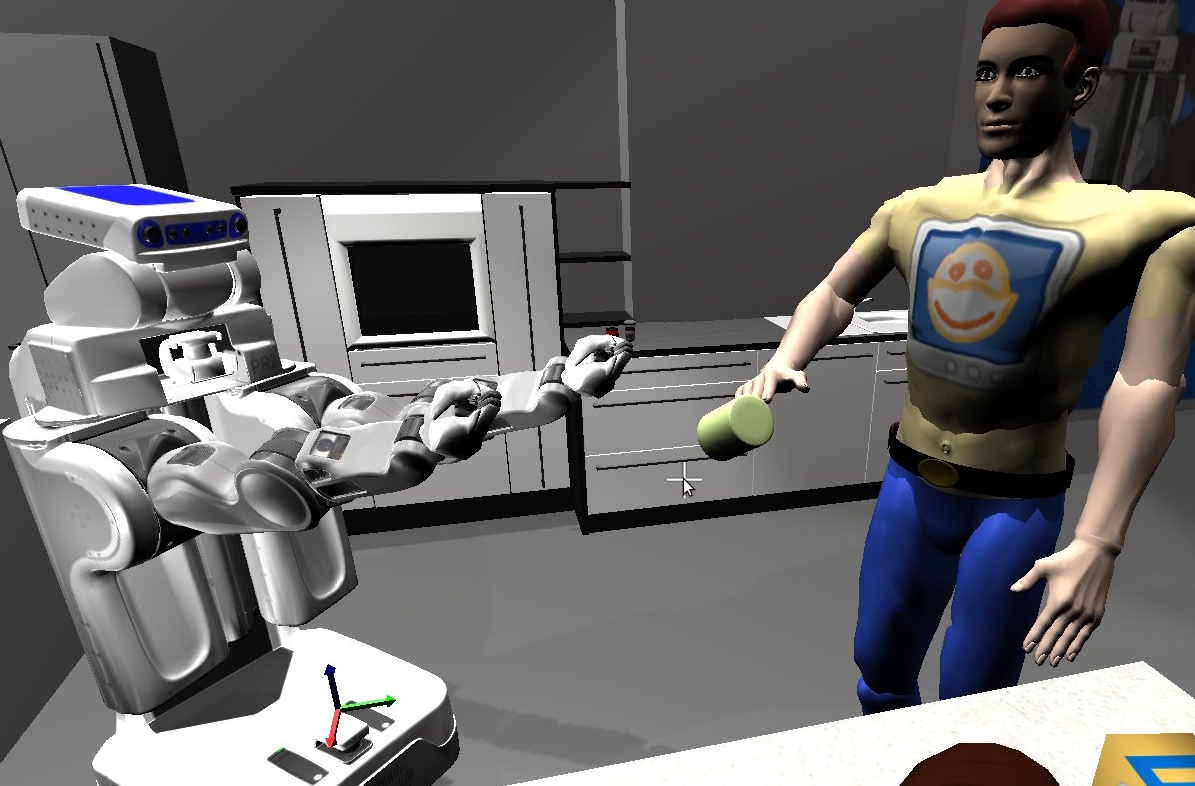
\includegraphics[width=0.9\linewidth]{morse_pr2.jpg}
      \caption{A PR2 and a human avatar in MORSE.}
      \label{fig|morse-hri}
\end{figure}

The MORSE components (sensors and actuators) exchange data with the robotics
software via middleware bindings (\emph{Software In The Loop} architecture).
Middlewares supported in the current version include ROS and YARP, as well as a
socket-based raw protocol. This design allows in principle to use the same
software in both the real robots and the simulator. Instructions given to the
robot are interpreted in the simulator to provide the control of actuators, such
as the motion of the robot and its arms.  The data from simulated sensors is
sent back through the middlewares, \eg exporting the images from cameras, or the
positions of the robot, human and other objects of interest.

MORSE also provides several features focused on human-robot
interaction~\cite{lemaignan2012morse} [...]

\section{Scenarios}
% Explain this section and introduce all use-cases

Lorem ipsum dolor sit amet, consectetuer adipiscing elit. Aenean commodo ligula
eget dolor. Aenean massa. Cum sociis natoque penatibus et magnis dis parturient
montes, nascetur ridiculus mus. Donec quam felis, ultricies nec, pellentesque
eu, pretium quis, sem. Nulla consequat massa quis enim. Donec pede justo,
fringilla vel, aliquet nec, vulputate eget, arcu. In enim justo, rhoncus ut,
imperdiet a, venenatis vitae, justo. Nullam dictum felis eu pede mollis pretium.
Integer tincidunt. Cras dapibus. Vivamus elementum semper nisi. Aenean vulputate
eleifend tellus. Aenean leo ligula, porttitor eu, consequat vitae, eleifend ac,
enim. Aliquam lorem ante, dapibus in, viverra quis, feugiat a, tellus. Phasellus
viverra nulla ut metus varius laoreet. Quisque rutrum. Aenean imperdiet. Etiam
ultricies nisi vel augue. Curabitur ullamcorper ultricies nisi. Nam eget dui.
Etiam rhoncus. Maecenas tempus, tellus eget condimentum rhoncus, sem quam semper
libero, sit amet adipiscing sem neque sed ipsum. Nam quam nunc, blandit vel,
luctus pulvinar, hendrerit id, lorem. Maecenas nec odio et ante tincidunt
tempus. Donec vitae sapien ut libero venenatis faucibus. Nullam quis ante. 

\subsection{Automated Execution of Prototype HRI Experiments}
\label{scenario1}

\emph{Use-Case:} In Human-Robot Interaction studies, robots often indicate
behavioral variability that may influence the experiment's final outcome.
However, manual testing on physical systems is usually the only way to prevent
this, but remains labour-intensive. To tackle this issue, we introduced
\emph{early automated prototype testing} \cite{2645922} that consists of: a
simulation environment, a software framework for automated bootstrapping of
prototype systems, execution verification of system components, automated result
assessment of experiments \cite{2563606} and a Continuous Integration (CI)
\cite{duvall2007continuous} server to centralize experiment execution. In our
setup we bootstrap and execute a simulated prototype system on a CI server and
assess the results in each run. In this particular scenario, a robot must report
the location of a virtual human in a domestic environment. Both, the robot and
the human, are moving about in the scene and meet in front of a table
(Figure~\ref{fig|proto}).

\begin{figure}[H]
      \centering
      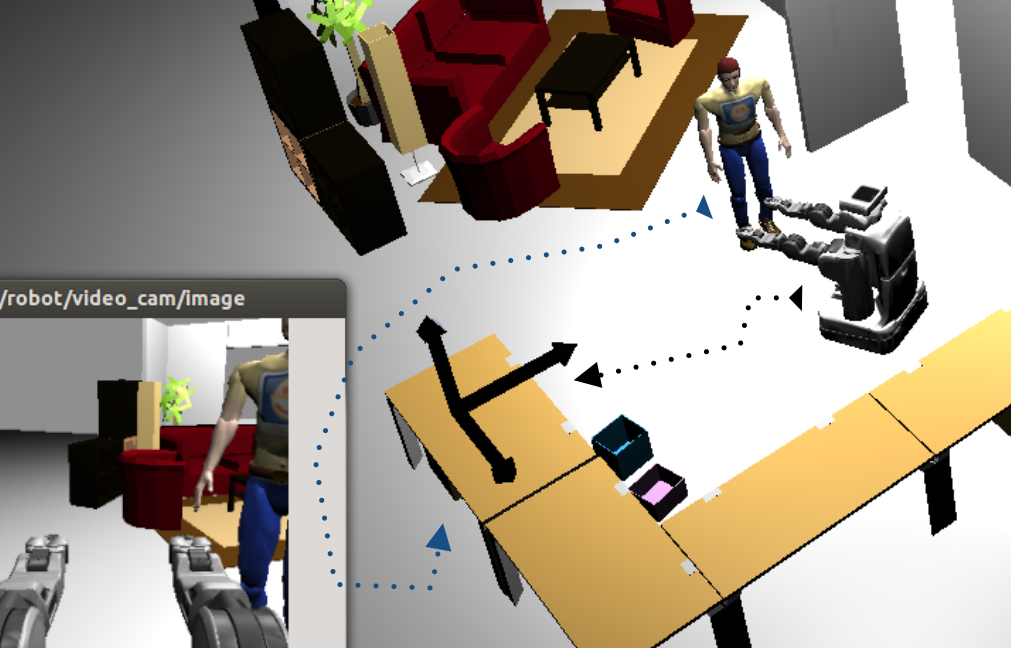
\includegraphics[width=0.9\linewidth]{proto-setup.png}
      \caption{Prototype HRI Simulation.}
      \label{fig|proto}
\end{figure}

The goal of this simulation setup is to incrementally decrease the level of
abstraction until a satisfactory/sufficient degree of ``realism'', to make an
assumption about real world behavior, is reached --- in an integrated and
continuous approach. In order to realise this goal, we make use of two essential
MORSE features: a) the human avatar that can be steered (set waypoints)
interactively via middleware and b) a semantic camera
\footnote{\url{openrobots.org/morse/doc/stable/user/sensors/semantic_camera.html}}
that extracts the location of a specific entity in the simulation environment.
The semantic camera is attached to the robot. If the human enters the robot's
field of view, the location is reported and sent via middleware. After each CI
run, the recorded movement trajectory of the human avatar is assessed (plotted)
and archived. We have explicitly chosen to simplify the extraction of the
human's location to acquire a ground truth in the first iterations of the
simulation. Based on the ground truth, we are able to exchange diverse
components, i.e., the semantic camera with a simulated laser scanner
\footnote{\url{openrobots.org/morse/doc/stable/user/sensors/laserscanner.html}},
to build a person hypothesis for instance, thus gradually develop, assess and
implement more complex scenarios. 

\emph{Contribution} The interactive avatar, semantic cam was extremely useful to
control, abstraction ...

\emph{Future requirements} Walking cycle, Pre-recorded activities (grasp,
loose), more than standing up, event based actions

\subsection{An Expectations Framework for Domestic Robot Assistants}
\label{scenario2}

In this scenario, an apartment is simulated in which a domestic service robot is
living together with a person. The robot is controlled via ROS and the CRAM
reactive plan language \cite{beetz2010cram}, which is used on many real robots
as well \cite{pancakes11humanoids}. The robots' duty is to observe the person
performing different activities and detect unexpected situations based on the
validation of different types of expectations \cite{Karg2013}. The detection of
such unexpected behavior can help future domestic service robots to better
assess situations and adapt their actions to human behavior. For this example,
the use of the MORSE simulator enabled us to set up a large, realistic testbed
by combining realistic robot control via the ROS middleware with the
unpredictability of human behavior using the human component of MORSE. Setting
up of such an apartment in a real-world setting would together with a suitable
sensor setup and a reliable robot control would not only introduce huge costs
but would also be a time-consuming task which can distract researchers from
their actual research focus. The use of the simulated scenario enables us to
gain many insights into the problem domain in a scenario that would not been
possible within our project and ultimately led to the successful validation of
the approach in a spatially limited real-world scenario.

\begin{figure}[H]
      \centering
      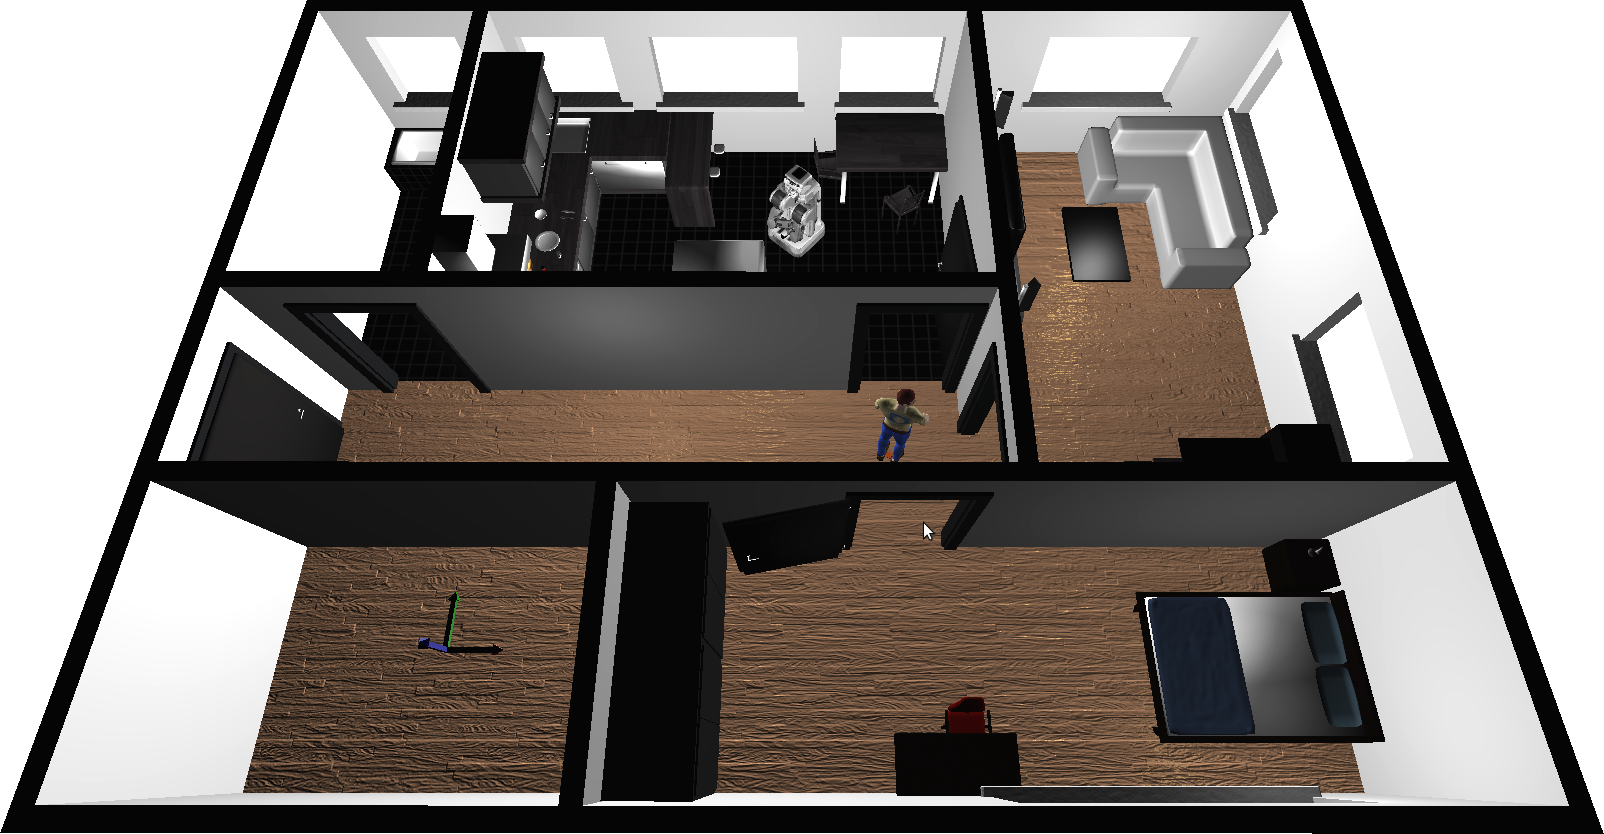
\includegraphics[width=0.9\linewidth]{morse_apartment.png}
      \caption{A simulated apartment with a domestic service robot and a person.}
      \label{fig|apartment}
\end{figure}

The human component of MORSE enabled us to test and validate our approach
dynamically in a variety of situations. Since it can be controlled in real-time
like in a 3D computer game while at the same time, a robot can be simulated by
state-of-the-art components, it is possible to generate a multitude of
situations on which the robot has to react. This greatly supported our project
to gain insights about our approach, detect weak points and make improvements.

\subsection{Data Acquisition through Automatic Scene Generation}
\label{scenario3}

Autonomous mobile robots that are to help and assist people in care homes,
households, and at other workplaces have to understand how activities performed
by humans affect the dynamics of objects in the environment. That is, they need
to know, when, where and how people manipulate objects and how they arrange and
structure them in space.

Within the STRANDS project\footnote{\url{http://www.strands-project.eu}} we are
generally aiming at understanding long-term, spatio-temporal relationships of
objects and activities of people. In the scenario described in this paper, we
looked in particular at learning qualitative spatial relations of objects on
office desks. As an accurate classification and pose estimation of objects on
real-world office desks is still a challenging and difficult task for current
robot perception systems we acquired a data set of object arrangements using
the MORSE simulator. For this, we first bootstrapped an object statistics from
manually labeled images of real office desks, and secondly, automatically
generated a set of physically possible desktop scenes (see
Figure~\ref{fig:simulated-desktop-scenes}, \cite{kunze14bootstrapping}). Based
on the generated data we learned relational models of object arrangements on
desks. The learnt models enable a robot to predict the position of an object
given a landmark. We employed these models to effectively guide a real robot in
object search tasks \cite{kunze14indirect} and evaluated its performance. The
automatic generation of object arrangements in simulation is not only useful
for the acquisition of data, but also for increasing the variability of scenes
in Human-Robot experiments in general. In future work we plan to use the
generated desktop scenes in web-applications to crowdsource Natural Language
descriptions of object arrangements and commands for robots from Internet
users.

\begin{figure}[tb]
  \centering
  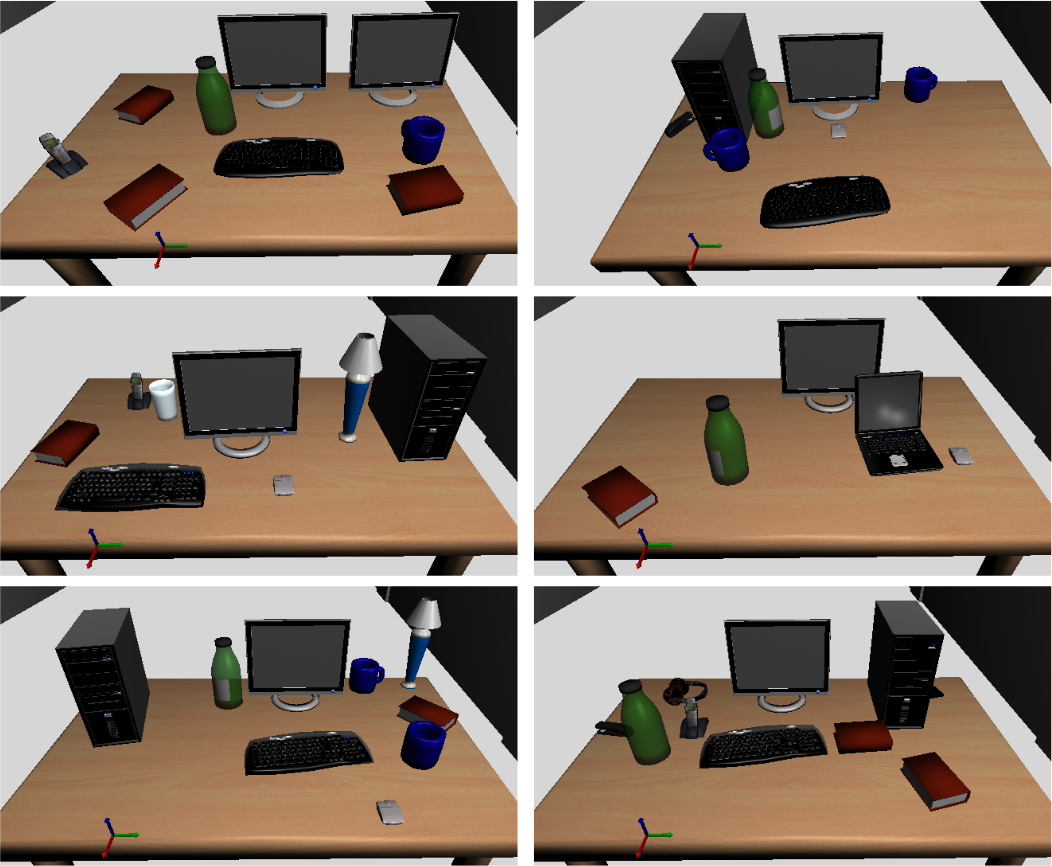
\includegraphics[width=.9\columnwidth]{figs/scenes.png}
  \caption{Automatically generated scenes of office desks.}
  \label{fig:simulated-desktop-scenes}
\end{figure}

\subsection{Scenario IV}
\label{scenario4}

Lorem ipsum dolor sit amet, consectetuer adipiscing elit. Aenean commodo ligula
eget dolor. Aenean massa. Cum sociis natoque penatibus et magnis dis parturient
montes, nascetur ridiculus mus. Donec quam felis, ultricies nec, pellentesque
eu, pretium quis, sem. Nulla consequat massa quis enim. Donec pede justo,
fringilla vel, aliquet nec, vulputate eget, arcu. In enim justo, rhoncus ut,
imperdiet a, venenatis vitae, justo. Nullam dictum felis eu pede mollis pretium.
Integer tincidunt. Cras dapibus. Vivamus elementum semper nisi. Aenean vulputate
eleifend tellus. Aenean leo ligula, porttitor eu, consequat vitae, eleifend ac,
enim. Aliquam lorem ante, dapibus in, viverra quis, feugiat a, tellus. Phasellus
viverra nulla ut metus varius laoreet. Quisque rutrum. Aenean imperdiet. Etiam
ultricies nisi vel augue. Curabitur ullamcorper ultricies nisi. Nam eget dui.
Etiam rhoncus. Maecenas tempus, tellus eget condimentum rhoncus, sem quam semper
libero, sit amet adipiscing sem neque sed ipsum. Nam quam nunc, blandit vel,
luctus pulvinar, hendrerit id, lorem. Maecenas nec odio et ante tincidunt
tempus. Donec vitae sapien ut libero venenatis faucibus. Nullam quis ante. 

\subsection{Scenario V}
\label{scenario5}

Lorem ipsum dolor sit amet, consectetuer adipiscing elit. Aenean commodo ligula
eget dolor. Aenean massa. Cum sociis natoque penatibus et magnis dis parturient
montes, nascetur ridiculus mus. Donec quam felis, ultricies nec, pellentesque
eu, pretium quis, sem. Nulla consequat massa quis enim. Donec pede justo,
fringilla vel, aliquet nec, vulputate eget, arcu. In enim justo, rhoncus ut,
imperdiet a, venenatis vitae, justo. Nullam dictum felis eu pede mollis pretium.
Integer tincidunt. Cras dapibus. Vivamus elementum semper nisi. Aenean vulputate
eleifend tellus. Aenean leo ligula, porttitor eu, consequat vitae, eleifend ac,
enim. Aliquam lorem ante, dapibus in, viverra quis, feugiat a, tellus. Phasellus
viverra nulla ut metus varius laoreet. Quisque rutrum. Aenean imperdiet. Etiam
ultricies nisi vel augue. Curabitur ullamcorper ultricies nisi. Nam eget dui.
Etiam rhoncus. Maecenas tempus, tellus eget condimentum rhoncus, sem quam semper
libero, sit amet adipiscing sem neque sed ipsum. Nam quam nunc, blandit vel,
luctus pulvinar, hendrerit id, lorem. Maecenas nec odio et ante tincidunt
tempus. Donec vitae sapien ut libero venenatis faucibus. Nullam quis ante. 

\section{Conclusion}
TODO

\section*{Acknowledgment}
TODO

\bibliographystyle{abbrv}
\bibliography{IROS-HRI}

\end{document}
